\begin{tikzpicture}[]

\node [anchor=south west] at (0, 0) {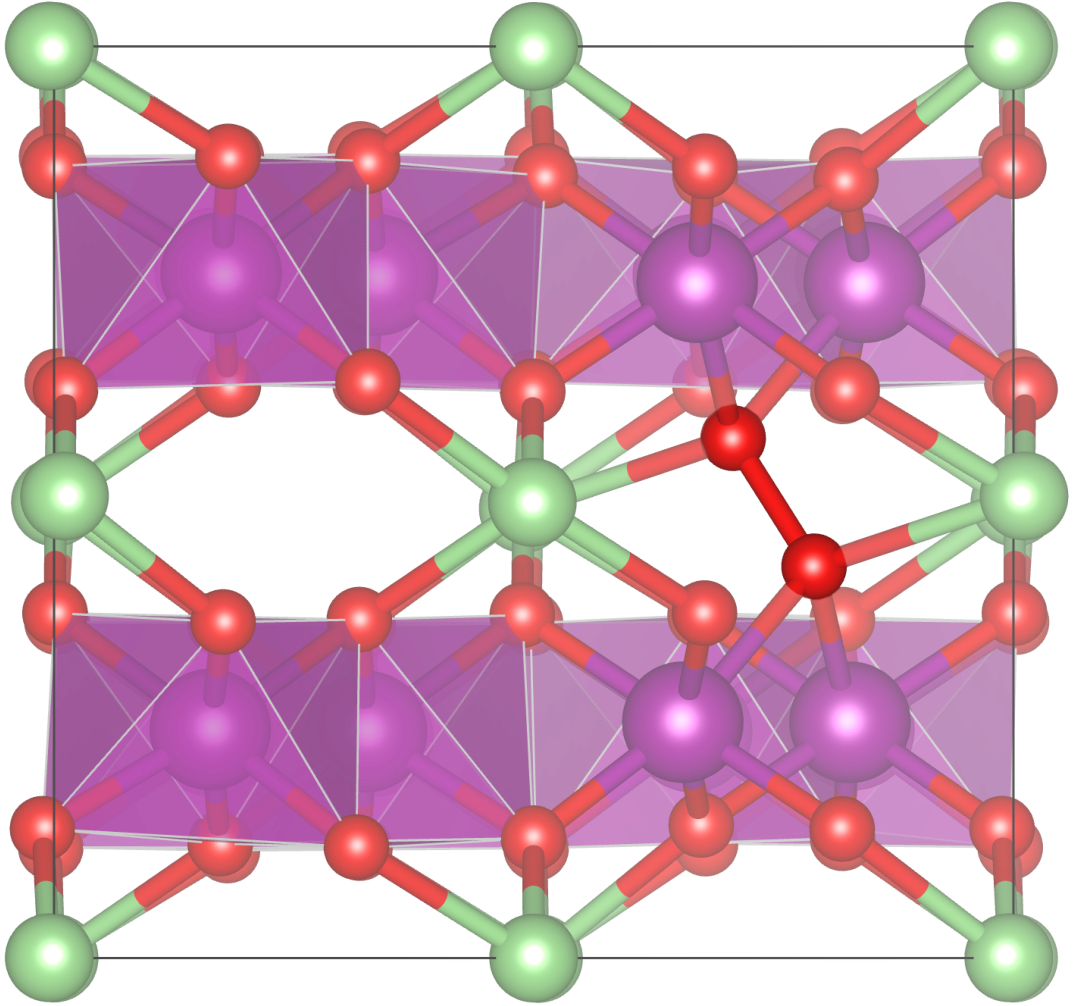
\includegraphics[height=0.3\textwidth]{\figurepath/batteries/Li2MnO3-d49_80.png}};

\coordinate (O1) at (4.01, 2.2);
\coordinate (O2) at (3.6, 2.85);
\node (distance) [fill=white, fill opacity=0.6, text opacity=1, rounded corners, font=\small] at (1.6, 2.5) {1.43 \si{\angstrom}};
\draw [<->, >=|, very thick] (O1) -- (O2);
\draw [-, thick] ($(O1)!0.5!(O2)$) -- (distance.east);

\begin{axis}[
height=5cm, 
width=0.4\textwidth, 
at={(0.45\textwidth, 3.3em)},
x dir=reverse,
xlabel={O-O Distance (\si{\angstrom})},
ylabel={Energy (meV)},
xticklabel={$\mathsf{\pgfmathprintnumber{\tick}}$},
yticklabel={$\mathsf{\pgfmathprintnumber{\tick}}$},
]

% This file was created by tikzplotlib v0.9.1.
\addplot [thick, black, dashed]
table {%
1.43041498524752 -553.091260000031
1.44041498524752 -551.377642628582
1.45041498524752 -546.431762921848
1.46041498524752 -538.54607949124
1.47041498524752 -528.013050948175
1.48041498524752 -515.125135904066
1.49041498524752 -500.174792970328
1.50041498524752 -483.454480758375
1.51041498524752 -465.256657879622
1.52041498524752 -445.873782945484
1.53041498524752 -425.598314567374
1.54041498524752 -404.722711356706
1.55041498524752 -383.539431924897
1.56041498524752 -362.340934883359
1.57041498524752 -341.419678843507
1.58041498524752 -321.018386344896
1.59041498524752 -301.150542620496
1.60041498524752 -281.763631502026
1.61041498524752 -262.805130781514
1.62041498524752 -244.222518250986
1.63041498524752 -225.963271702471
1.64041498524752 -207.974868927997
1.65041498524752 -190.204787719591
1.66041498524752 -172.600505869281
1.67041498524752 -155.109501169094
1.68041498524752 -137.679251411059
1.69041498524752 -120.257234387202
1.70041498524752 -102.790927889552
1.71041498524752 -85.2278097101362
1.72041498524752 -67.5153576409824
1.73041498524752 -49.6010494741182
1.74041498524752 -31.4323630015713
1.75041498524752 -12.9567760153694
1.76041498524752 5.87823369245977
1.77041498524752 25.124203929812
1.78041498524752 44.7651207939874
1.79041498524752 64.6750691859931
1.80041498524752 84.7180456287522
1.81041498524752 104.758046645188
1.82041498524752 124.659068758223
1.83041498524752 144.28510849078
1.84041498524752 163.500162365784
1.85041498524752 182.168226906156
1.86041498524752 200.153298634819
1.87041498524752 217.319374074698
1.88041498524752 233.530449748714
1.89041498524752 248.650522179791
1.90041498524752 262.543587890852
1.91041498524752 275.073643404821
1.92041498524752 286.104685244619
1.93041498524752 295.50070993317
1.94041498524752 303.125713993398
1.95041498524752 308.843693948225
1.96041498524752 312.518646320574
1.97041498524752 314.014567633369
1.98041498524752 313.398597500051
1.99041498524752 311.053533252383
2.00041498524752 307.13022917784
2.01041498524752 301.773806636548
2.02041498524752 295.129386988631
2.03041498524752 287.342091594215
2.04041498524752 278.557041813427
2.05041498524752 268.919359006392
2.06041498524752 258.574164533235
2.07041498524752 247.666579754083
2.08041498524752 236.341726029061
2.09041498524752 224.744724718295
2.10041498524752 213.020697181911
2.11041498524752 201.314764780033
2.12041498524752 189.772048872789
2.13041498524752 178.537670820304
2.14041498524752 167.756751982704
2.15041498524752 157.574413720114
2.16041498524752 148.134379241703
2.17041498524752 139.505115028043
2.18041498524752 131.643149700525
2.19041498524752 124.495913025972
2.20041498524752 118.010834771208
2.21041498524752 112.135344703057
2.22041498524752 106.816872588343
2.23041498524752 102.00284819389
2.24041498524752 97.6407012865209
2.25041498524752 93.6778616330605
2.26041498524752 90.0617590003324
2.27041498524752 86.7398231551602
2.28041498524752 83.6594838643678
2.29041498524752 80.7681708947793
2.30041498524752 78.0133140132184
2.31041498524752 75.3423429865087
2.32041498524752 72.7111848560701
2.33041498524752 70.1329170892376
2.34041498524752 67.6441771638725
2.35041498524752 65.2816761285648
2.36041498524752 63.0821250319044
2.37041498524752 61.0822349224814
2.38041498524752 59.3187168488857
2.39041498524752 57.8282818597072
2.40041498524752 56.6476410035358
2.41041498524752 55.8135053289616
2.42041498524752 55.3591156502156
2.43041498524752 55.0730147158313
2.44041498524752 54.3418496115398
2.45041498524752 52.5149106078037
2.46041498524752 48.941487975086
2.47041498524752 43.0266663682665
2.48041498524752 35.0638700443965
2.49041498524752 26.0588023425712
2.50041498524752 17.0372094540019
2.51041498524752 9.02483756989976
2.52041498524752 3.04743288147699
2.53041498524752 0.130741579945283
};
\addplot [thick, red, mark=*, mark size=2, mark options={solid}, only marks]
table {%
2.53289368015598 0
2.46457000294431 46.7890599999805
2.41729780104295 55.45982000001
2.31211857608837 74.8918900000035
2.15692701821804 151.334410000004
1.97196758439653 314.042639999968
1.76726251651896 19.0099999999802
1.57088682042962 -340.444320000017
1.43041498524752 -553.091260000031
};


\end{axis}

\node [font=\bfseries, anchor=north west] at (7.2, 4.6) {A};

\node (fig2) [anchor=south east] at (0.95\textwidth, -13em) {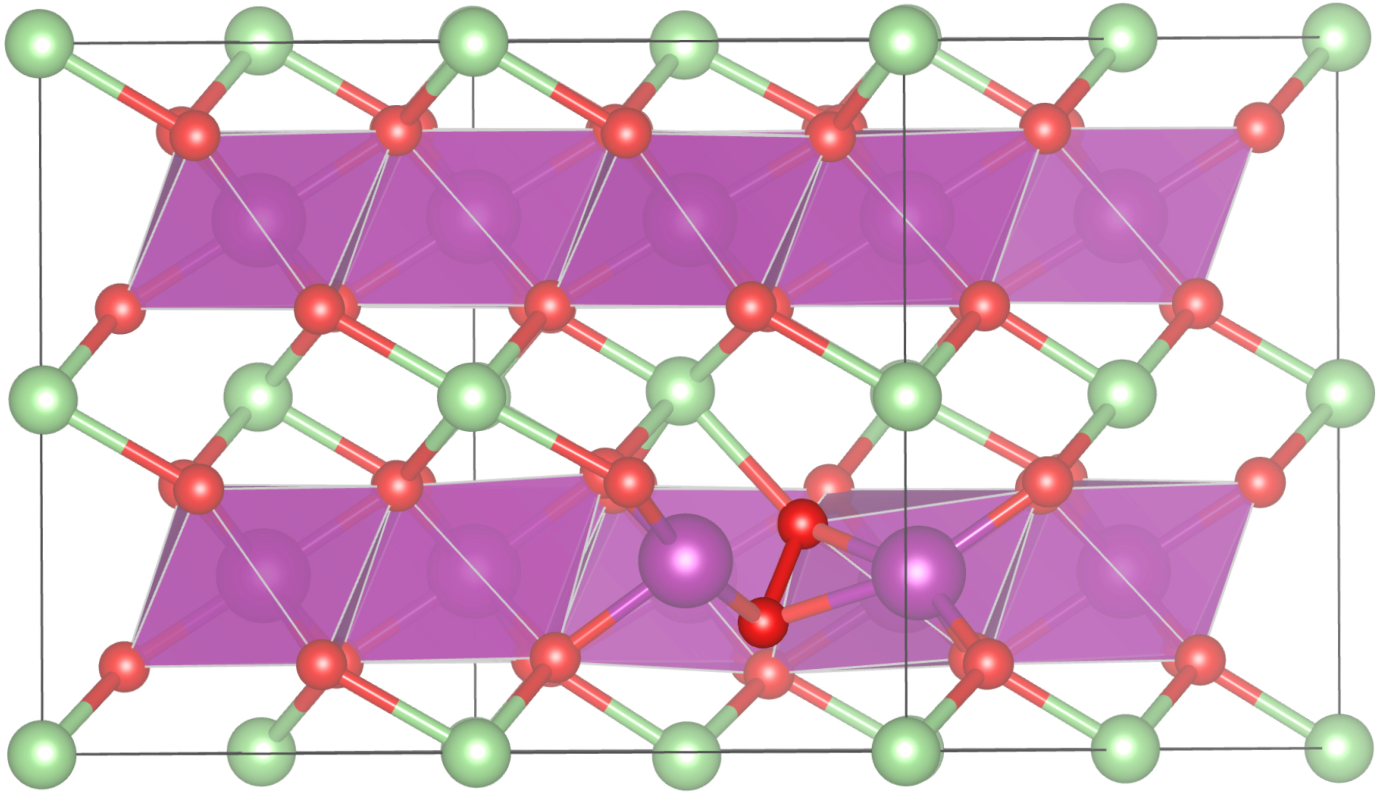
\includegraphics[height=0.3\textwidth]{\figurepath/batteries/Li2MnO3-d48_92.png}};

\coordinate (O1) at ($(fig2) + (0.705, -0.75)$);
\coordinate (O2) at ($(fig2) + (0.44, -1.39)$);
\node (distance) [
font=\small, fill=white, fill opacity=0.6, text opacity=1, rounded corners
] at (14, -3.5) {1.46 \si{\angstrom}};
\draw [<->, >=|, very thick] (O1) -- (O2);
\draw [-, thick] ($(O1)!0.5!(O2)$) -- (distance);

\begin{axis}[
height=5cm, 
width=0.4\textwidth, 
at={(0.1\textwidth, -9.7em)},
x dir=reverse,
xlabel={O-O Distance (\si{\angstrom})},
ylabel={Energy (meV)},
xticklabel={$\mathsf{\pgfmathprintnumber{\tick}}$},
yticklabel={$\mathsf{\pgfmathprintnumber{\tick}}$},
]

% This file was created by tikzplotlib v0.9.1.
\addplot [thick, black, dashed]
table {%
1.4566494053843 -82.8172899999799
1.4666494053843 -81.2560763673107
1.4766494053843 -76.7947268149007
1.4866494053843 -69.7666783611462
1.4966494053843 -60.5053680244437
1.5066494053843 -49.3442328231896
1.5166494053843 -36.6167097757802
1.5266494053843 -22.6562359006121
1.5366494053843 -7.79624821608146
1.5466494053843 7.65847202609837
1.5566494053843 23.5899600898859
1.5666494053843 39.9551223502687
1.5766494053843 56.7110651744154
1.5866494053843 73.8148949294948
1.5966494053843 91.2237179826755
1.6066494053843 108.894640701126
1.6166494053843 126.784769452016
1.6266494053843 144.851210602513
1.6366494053843 163.051070519786
1.6466494053843 181.341455571004
1.6566494053843 199.679472123335
1.6666494053843 218.022226543949
1.6766494053843 236.326825200013
1.6866494053843 254.550374458698
1.6966494053843 272.64998068717
1.7066494053843 290.5827502526
1.7166494053843 308.305789522155
1.7266494053843 325.776204863005
1.7366494053843 342.951102642318
1.7466494053843 359.787589227262
1.7566494053843 376.242770985008
1.7666494053843 392.275847347668
1.7766494053843 407.857689302546
1.7866494053843 422.96321199675
1.7966494053843 437.567334526386
1.8066494053843 451.644975987557
1.8166494053843 465.171055476366
1.8266494053843 478.120492088916
1.8366494053843 490.468204921312
1.8466494053843 502.189113069657
1.8566494053843 513.258135630055
1.8666494053843 523.650191698609
1.8766494053843 533.340200371423
1.8866494053843 542.303080744601
1.8966494053843 550.513751914245
1.9066494053843 557.947132976461
1.9166494053843 564.57814302735
1.9266494053843 570.381701163017
1.9366494053843 575.332726479567
1.9466494053843 579.406138073101
1.9566494053843 582.576855039724
1.9666494053843 584.819796475539
1.9766494053843 586.10988147665
1.9866494053843 586.390403545011
1.9966494053843 584.489733791969
2.0066494053843 579.980430115906
2.0166494053843 573.074663703546
2.0266494053843 563.984605741615
2.0366494053843 552.922427416838
2.0466494053843 540.100299915941
2.0566494053843 525.730394425649
2.0666494053843 510.024882132686
2.0766494053843 493.195934223779
2.0866494053843 475.455721885652
2.0966494053843 457.016416305032
2.1066494053843 438.090188668641
2.1166494053843 418.889210163206
2.1266494053843 399.625651975454
2.1366494053843 380.511685292108
2.1466494053843 361.759481299893
2.1566494053843 343.581211185535
2.1666494053843 326.189046135761
2.1766494053843 309.793704112122
2.1866494053843 294.506612795319
2.1966494053843 280.277909230181
2.2066494053843 267.042954730596
2.2166494053843 254.73711061045
2.2266494053843 243.295738183629
2.2366494053843 232.654198764022
2.2466494053843 222.747853665516
2.2566494053843 213.512064201998
2.2666494053843 204.882191687355
2.2766494053843 196.793597435474
2.2866494053843 189.181642760244
2.2966494053843 181.981688975551
2.3066494053843 175.129097395282
2.3166494053843 168.559229333324
2.3266494053843 162.207446103566
2.3366494053843 156.009109019893
2.3466494053843 149.899579396194
2.3566494053843 143.814517236325
2.3666494053843 137.714015193111
2.3766494053843 131.600347923166
2.3866494053843 125.479973967742
2.3966494053843 119.359351868087
2.4066494053843 113.244940165453
2.4166494053843 107.143197401088
2.4266494053843 101.060582116243
2.4366494053843 95.0035528521679
2.4466494053843 88.9785681501126
2.4566494053843 82.9920865513269
2.4666494053843 77.0505665970607
2.4766494053843 71.160466828564
2.4866494053843 65.3282457870872
2.4966494053843 59.56036201388
2.5066494053843 53.863274050192
2.5166494053843 48.2467496563142
2.5266494053843 42.7433675729223
2.5366494053843 37.3953200687798
2.5466494053843 32.2448331135497
2.5566494053843 27.3341326768954
2.5666494053843 22.7054447284804
2.5766494053843 18.4009952379677
2.5866494053843 14.4630101750202
2.5966494053843 10.9337155093015
2.6066494053843 7.85533721047477
2.6166494053843 5.27010124820321
2.6266494053843 3.22023359214989
2.6366494053843 1.73915479787467
2.6466494053843 0.772752158584978
2.6566494053843 0.216767002869623
2.6666494053843 -0.0336518700062289
2.6766494053843 -0.0833556607773805
2.6866494053843 -0.0371955701786719
};
\addplot [thick, red, mark=*, mark size=2, mark options={solid}, only marks]
table {%
2.69644801919029 0
2.62954078608243 2.73332000000437
2.50843083366394 52.8562999999735
2.35371734388973 145.599790000006
2.17349124489821 314.85189
1.98479888323523 586.43914999999
1.7577491767086 378.027349999968
1.53825382424304 -5.35070000000815
1.4566494053843 -82.8172899999799
};


\end{axis}
\node [font=\bfseries, anchor=north west] at (1.65, -0.4) {E};


\node [anchor=south east] at (0.95\textwidth, 3em) {%
\begin{tabular}{lr}
\multicolumn{2}{c}{$\Delta E$ (meV)} \\\hline
\textbf{A} & -553 \\
\textbf{B} & +67 \\
\textbf{C} & $\rightarrow$ \textbf{E} \\
\textbf{D} & +338 \\
\textbf{E} & -83 \\
\textbf{F} & +320 \\
\hline
\end{tabular}
};

\end{tikzpicture}
